% Document class and two-column conversion
\documentclass[twocolumn]{report}
% dimensions of paper and relative text positioning
\usepackage[a4paper,top=2cm,bottom=2cm,left=2cm,right=2cm]{geometry}
% math symbols
\usepackage{amsmath}
\usepackage{amssymb}
% package for including URLs
\usepackage{url}
% Required for including images
\usepackage{graphicx}
\usepackage{float} % Required for specifying the exact location of a figure

% enable writing in greek
\usepackage[greek,english]{babel}
\usepackage[utf8]{inputenc}

\setlength{\parindent}{0pt} % Removes all indentation from paragraphs

% Start of the document
\begin{document}

% Set the language to greek
\selectlanguage{greek}

% Title page
\title{\Huge \bfseries Τεχνικές Βελτιστοποίησης \\ \selectlanguage{english}Project 2024\selectlanguage{greek}} %\Huge and \bfseries are used to make the title bigger and bold
\author{Παπαδάκης Κωνσταντίνος Φώτιος\vspace{0.5cm} \\  ΑΕΜ:10371} % \vspace{0.5cm} is used to add some vertical space between the author and the AEM
\date{\today}
% prints the title, author and date on a separate page
\maketitle

% General introduction
\section*{Γενετικοί Αλγόριθμοι}
Οι γενετικοί αλγόριθμοι είναι μια κατηγορία αλγορίθμων βελτιστοποίησης οι
οποίοι εμπνέονται από τον μηχανισμό της εξέλιξης που συναντάμε στη φύση.
Ξεκινάμε με ένα πληθυσμό από διαφορετικές λύσεις του προβλήματος και έπειτα, 
ύστερα από διάφορες τυχαίες μεταλλάξεις και διασταυρώσεις αυτών, επιλέγουμε 
τη βέλτιστη απάντηση ως λύση του προβλήματος μας.
\begin{figure}[H]
    \centering
    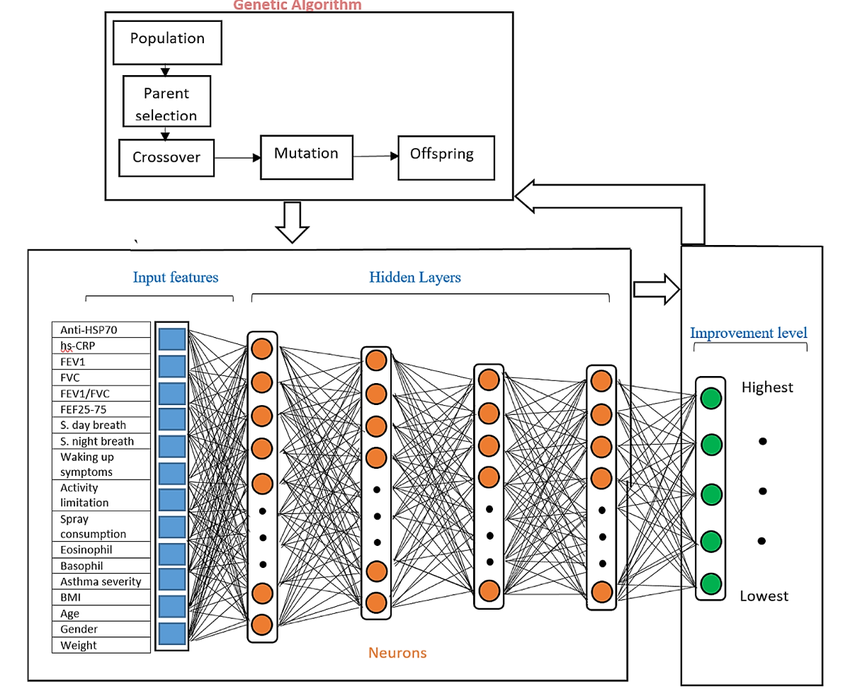
\includegraphics[width=0.4\textwidth]{media/genetic_algorithm.png}
    \caption{Γενετικός Αλγόριθμος}
\end{figure}

% Mathematical formulation
\section*{Θέμα 1\\Μαθηματική Διατύπωση}
Να δοθεί η μαθηματική διατύπωση του προβλήματος.
\subsection*{Λύση}


% Genetic Algorithm
\section*{Θέμα 2\\Γενετικός Αλγόριθμος}
Να υλοποιηθεί ένας γενετικός αλγόριθμος στο \selectlanguage{english}
Matlab\selectlanguage{greek} που να λύνει το πρόβλημα.
\subsection*{Λύση}


% Alternate 
\section*{Θέμα 3\\Μεταβαλλόμενο \selectlanguage{english}V\selectlanguage{greek}}
Θεωρήστε ότι ο ρυθμός εισερχομένων οχημάτων $V$ μπορεί να μεταβάλλεται μέχρι 
$\pm 15\%$ της αρχικής του τιμής. Να επιλυθεί το πρόβλημα εκ νέου με 
την ίδια μεθοδολογία βελτιστοποίησης. 
\subsection*{Λύση}

% Comments
\section*{Σχόλια}

% End of the document
\end{document}